\documentclass[11pt,a4paper,bibtotocnumbered]{scrreprt}		                                   

\usepackage{graphicx}
\usepackage[dvipsnames]{xcolor}
\usepackage{a4}
\usepackage[onehalfspacing]{setspace}
\usepackage[ngerman]{babel}
\usepackage[utf8]{inputenc}
\usepackage{amsmath}
\usepackage{caption}
\usepackage{tabularx}
\usepackage{listings}
\usepackage[babel,german=quotes]{csquotes}
\usepackage[printonlyused]{acronym}
\usepackage[linktoc=all, hidelinks]{hyperref}

\renewcaptionname{ngerman}\figureautorefname{Abb.}

\captionsetup[table]{belowskip=8pt}


\newcommand{\thema}{Eine domänenspezifische Sprache für die Dialogische Logik}
\newcommand{\abgabedatum}{24.07.2015}
\newcommand{\zusammenfassung}{d}


\begin{document}



% ============================ FRONT MATTER
\pagenumbering{roman}
\begin{singlespace}
\begin{titlepage}

\vspace*{-3.5cm}

\begin{flushleft}
\hspace*{-1cm} 
\includegraphics[width=15.7cm]{htwg-logo}
\end{flushleft}

\vspace{2.5cm}

\begin{center}
	\huge{
		\textbf{\thema} \\[5cm]
	}
	\Large{
		\textbf{Tobias Keh, Simon Kessler}} \\[6.5cm]
	\large{
		\textbf{Konstanz, \abgabedatum} \\[2.3cm]
	}
	
	\Huge{
		\textbf{{\sf SEMINARARBEIT}}
	}
\end{center}

\end{titlepage}
\setcounter{page}{1}
\begin{center}
{\Large \textbf{Zusammenfassung (Abstract)}}
\end{center}

\bigskip

\begin{center}
	\begin{tabular}{p{2.8cm}p{10cm}}
		Thema: & \thema \\
		 & \\
		Abgabedatum: & \abgabedatum \\
		 & \\
	\end{tabular}
\end{center}

\bigskip

\noindent
\zusammenfassung
\end{singlespace}


\tableofcontents
\listoffigures
\listoftables

\chapter*{Abkürzungsverzeichnis} 

% Alphabetisch sortieren
\begin{acronym}[LAENGE]
\acro{EBNF}{Erweiterte Backus-Naur-Form}
\end{acronym}

\cleardoublepage
% ============================ ENDE FRONT MATTER



% ============================ HAUPTTEIL THESIS
\pagenumbering{arabic}


% ============================ CHAPTER
\chapter{Einleitung} % Simon

Die Demokratie wandelt sich und versucht sich neu zu erfinden. 
Konzepte wie die \emph{deliberative Demokratie} erhalten unter dem Schlagwort \emph{Demokratie 2.0} neuen Zulauf. 
Auch die zunehmende Vernetzung der Gesellschaft durch das Internet trägt zu diesem Trend bei. 
Während in einer nicht vernetzten Welt Bürger nur sehr wenige Berührungs- und Einflusspunkte mit der Politik haben (z. B. während den Wahlen), kann das Internet helfen, Bürger aktiv in die politische und demokratische Entscheidungsfindung einzubeziehen.
Auch als \emph{Liquid Democracy} bekannt, ermöglicht dieser Ansatz es den Bürgern, für einzelne Gesetze abzustimmen und Argumente einzubringen bzw. Diskussionen zu führen.
Die Diskussionen folgen bisher einem unstrukturierten Ablauf von Argumenten.
Hier könnte die \emph{dialogische Logik} zu einem geordneten, gesteuerten und fairen Dialog verhelfen.

Da die Regeln der dialogischen Logik und ihre formale Darstellung zwar klar und deutlich sind, so verhindern sie doch den Zugang der breiten Masse zu diesem Werkzeug.
Oder wie Ludwig Wittgenstein einst formulierte:
\begin{quote}
\enquote{Die Grenzen meiner Sprache bedeuten die Grenzen meiner Welt.}
\end{quote}
Das heißt, wollen wir wirklich Bürger einer Demokratie 2.0 ausgrenzen, die diese neue und innovative Form des Dialogs nicht beherrschen? Oder wollen wir Wege finden, auch diesen Menschen den dialogischen Dialog zu ermöglichen?

In dieser Projektarbeit soll deshalb eine domänenspezifische Sprache entwickelt werden, die es ermöglicht einen dialogischen Dialog mit annähernd natürlichsprachlichen Elementen zu formulieren. 
Dabei liegt der Fokus auf einer einfachen Erlernbarkeit der Sprache.

Die Arbeit gliedert sich in eine weitere Motivation für die Arbeit, Erläuterung der theoretischen Grundlagen, Definition der Syntax, Evaluierung von Anwendungsfällen und einem abschließenden Fazit und Ausblick.
Es erfolgt eine Beschränkung auf die Syntax der Sprache, wobei anwendungsspezifische Beispiele für die semantische Auswertung genannt werden.

% ============================ CHAPTER
\chapter{Motivation} % Tobi


% ============================ CHAPTER
\chapter{Theoretische Grundlagen}  % Tobi

\section{Dialogische Logik}

%Vlt noch "Why Interaction is more powerful...." zitieren?

\section{Domänenspezifische Sprachen} 

\subsection{Interne DSL}

\subsection{Externe DSL}

\section{Grammatiken} 
Chomsky, etc.

\section{Werkzeugunterstützung} 

% ============================ CHAPTER
\chapter{Die Sprache \enquote{Logic}} % Simon

In diesem Kapitel soll die entwickelte Sprache \enquote{Logic} mit ihrer Grammatik und Beispielen vorgestellt werden.
Ziel der Sprache ist es, eine Brücke zwischen der Semantik und der Syntax Ebene zur maschinellen Verarbeitung zu bilden (vgl. \cite[Folie 11]{OrtnerDL}).
Dabei soll das \enquote{Gemeinte} möglichst simpel in der formalen dialogischen Logik ausgedrückt werden können.

\section{Meta-Modell}

Die Sprache basiert auf einem Meta-Modell, welches es erlaubt, die einzelnen Elemente der Sprache maschinell in anderen Anwendungen zu verarbeiten.
In \autoref{metamodell} ist das verwendete Meta-Modell ersichtlich.

\begin{figure}[htbp]
\centering
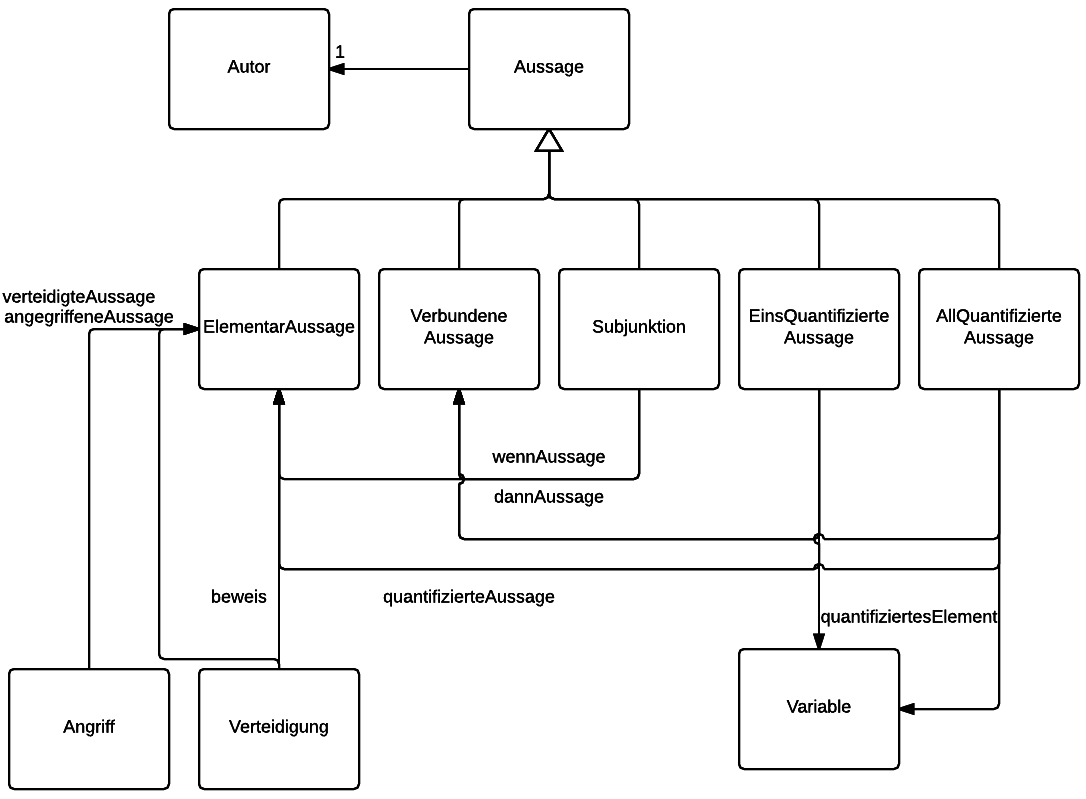
\includegraphics[width=1\textwidth]{img/metamodell.png}
\caption{Meta-Modell von \enquote{Logic}}
\label{metamodell}
\end{figure}

Jede Aussage besitzt exakt einen Autor, der namentlich genannt wird.
Dies ist wichtig, um im Dialog eine eindeutige Zuweisung von Aussagen vornehmen und entsprechend referenzieren zu können.
Eine Aussage wiederum ist im konkreten Fall ein Typ aus der Menge \{ElementarAussage, VerbundeneAussage, Subjunktion, EinsQuantifizierteAussage, AllQuantifizierteAussage\}. 
ElementarAussage besitzt ein Attribut mit dem Inhalt der Aussage als Textform.
Der Typ VerbundeneAussage besteht aus einer ElementarAussage und einer weiteren Aussage, verbunden durch ein Schlüsselwort (Adjunktor oder Konjunktor).
Auch die Quantifizierung von Aussagen wird unterstützt, da dies einige weitere Anwendungsfälle eröffnet.
Eine quantifizierte Aussage assoziiert eine Variable (Text), die entsprechend quantifiziert wird und eine Aussage, für welche die Variable gebunden wird.
Subjunktionen referenzieren eine ElementarAussage über das Attribut \enquote{wenn} und eine VerbundeneAussage oder ElemtarAussage über das Attribut \enquote{dann}.
Dies entspricht dem folgenden Schema: \enquote{wenn} $\rightarrow$ \enquote{dann}.
Auch die Angriffe und Verteidigungen im dialogischen Dialog finden sich im Meta-Modell wieder. 
Diese beziehen sich stets auf ein Objekt des Typs ElementarAussage.
Die Verteidigung referenziert dabei sowohl die verteidigte Aussage als auch eine Aussage, die als Beweis dient.

Um Formulierungen verständlich und nicht zu komplex werden zu lassen, wurden gewisse Einschränkungen vorgenommen. 
So können in einer Subjunktion keine weiteren Subjunktionen verschachtelt werden.
Eine Aussage wie z. B. \enquote{wenn $\rightarrow$ (wenn $\rightarrow$ dann)} ist somit ausgeschlossen.
Solche Konstrukte kommen in Dialogen aber recht selten vor und stellen nur eine unwesentliche Einschränkung dar.
Diese Einschränkungen fördern das einfache Verständnis von Dialogen und verhindern, dass kompliziert geschachtelte Formulierungen verwendet werden, die den Bürgern unter Umständen nicht verständlich sind.

\section{Grammatik}

Unser Vorschlag für die konkrete Syntax, um das Meta-Modell abzubilden ist in \autoref{grammatik} ersichtlich.
Die Notation ist an die \ac{EBNF} angelehnt und beschreibt die Grammatik für das Tool Xtext \cite{Xtext}.

\begin{table}[htbp]
\centering
\caption{Wichtige Terminale der DSL}
\label{terminale}
\begin{tabularx}{\textwidth}{|p{3cm}|X|}
\hline
« 				& Öffnendes Symbol für eine Elementaraussage.  \\ \hline
» 				& Schließendes Symbol für eine Elementaraussage.  \\ \hline
und  			& Konjunktion zwischen zwei Aussagen.   \\  \hline
oder  		& Adjunktion zwischen zwei Aussagen.   \\  \hline
.     			& Schließt eine Aussage.   \\  \hline
:				& Schließt die Nennung des Autors.   \\  \hline
wenn, weil	& Öffnet in einer Subjunktion den \enquote{Wenn}-Teil.   \\  \hline
dann, folgt daraus	& Leitet in einer Subjunktion den \enquote{Wenn}-Teil ein.   \\  \hline
für mindestens einen, eine, ein & Einsquantifiziert eine Variable (Text).   \\  \hline
für alle & Allquantifiziert eine Variable (Text).   \\  \hline
gilt:				& Öffnet die Definition einer Aussage, auf die sich die quantifizierte Variable bezieht.   \\  \hline
Ich bezweifle:		& Eröffnet einen Angriff auf eine Elementaraussage.   \\  \hline
Ich beweise:		& Eröffnet eine Verteidigung einer Elementaraussagen.   \\  \hline
durch:		& Leitet die Nennung einer Elementar oder verbundenen Aussage ein, die als Beweis in einer Verteidigung dient.   \\  \hline
\end{tabularx}
\end{table}

Wichtige Terminale sind in \autoref{terminale} ersichtlich.
Es wurden explizit Wörter und Zeichen gewählt die einerseits beim Lesen einer Aussage nicht stören und den natürlichsprachlichen Eindruck so wenig wie möglich beeinträchtigen. Andererseits aber auch eine klare Struktur bieten, um Aussagen auch ohne Tool-Unterstützung schnell erfassen bzw. formulieren zu können.

Da in der deutschen Sprache Guillemets («,») recht selten verwendet werden, trotzdem im Lesefluss kaum stören, bieten sich diese gut als \enquote{Klammer} für Aussagen an.
So können auch weiterhin normale Anführungszeichen in Aussagen vorkommen.
Durch die generischen Terminale für Subjunktionen, Quantoren, Angriffe und Verteidigungen ist sichergestellt, dass für eine Vielzahl von Aussagen ein annähernd korrekter deutscher Satz entsteht, der sich flüssig lesen lässt.


\begin{figure}[htbp]
\centering
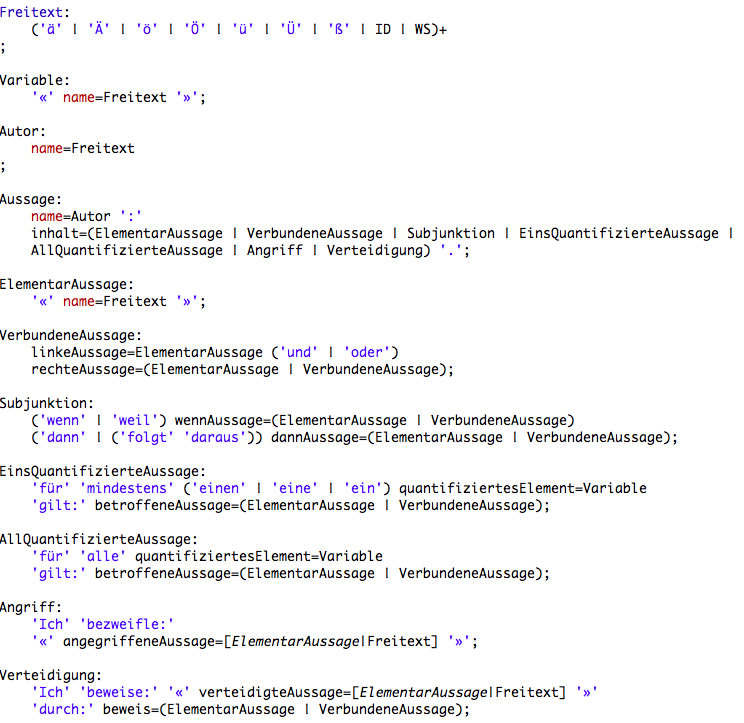
\includegraphics[width=1\textwidth]{img/grammatik.png}
\caption{Grammatik von \enquote{Logic}}
\label{grammatik}
\end{figure}


ECLIPSE TREE!

\section{Beispiele}

Nachfolgend soll die Grammatik der Sprache mit Beispielen verdeutlicht werden.
Zuerst werden einfache logische Ausdrücke vorgestellt, die dann angegriffen bzw. verteidigt werden und abschließend in einem vollständigen Beispieldialog münden.

\subsection{Logische Aussage}

Eine einfache Aussage, wie z. B. \enquote{Die Politik hat versagt} (Max Muster) lassen sich mit der DSL als \enquote{Max Muster: «Die Politik hat versagt».} ausdrücken.
Zusammengesetzte Aussagen werden wie folgt formuliert: \enquote{Max Muster: «Die Politk hat versagt» und «das Volk ist politikverdrossen».}.
Die Subjunktion könnte so verwendet werden: \enquote{Max Muster: weil «das Volk politikverdrossen ist» folgt daraus «dass die Politk versagt hat».}
Quantifizierung von Variablen ist praktisch für verallgemeinernde Aussagen, wie \enquote{Max Muster: für alle «Jugendlichen» gilt: «dass sie nicht wissen, was sie einmal arbeiten möchten».}

\subsection{Angriff und Verteidigung}

Insbesondere der strukturierte Ablauf von Diskussionen lässt sich mit der dialogischen Logik hervorragend unterstützen. Deshalb sollen nachfolgend einige Beispiele für einen Angriff bzw. eine Verteidigung folgen.
Beispiel Angriff: \enquote{Petra Maier: Ich bezweifle «das Volk politikverdrossen ist».}
Eine Verteidigung könnte lauten: \enquote{Max Muster: Ich beweise «das Volk ist politikverdrossen» durch: «die Wahlbeteiligung sinkt seit den letzten zehn Jahren kontinuierlich».}

\subsection{Gesamtdialog}

Nachfolgend wird eine Diskussion um die Sperrstunde in der Konstanzer Innenstadt mit Hilfe der dialogischen Logik und der DSL \enquote{Logic} geführt. 
Alle Namen und Argumente sind rein fiktiv.

Michaela P. (Anwohnerin): für alle «Anwohner in der Innenstadt» gilt: «die Sperrstunde um 3 Uhr raubt uns den Schlaf» und «führt zu mehr Vandalismus durch die Betrunkenen».\\
Jonas F. (Student): Ich bezweifle «führt zu mehr Vandalismus durch die Betrunkenen».\\
Michaela P. (Anwohnerin): Ich beweise «führt zu mehr Vandalismus durch die Betrunkenen» durch: «die Polizeistatistik von 2014, die einen klaren Zusammenhang herstellt». \\
Jonas F. (Student): Ich bezweifle «die Sperrstunde um 3 Uhr raubt uns den Schlaf».\\
Michaela P. (Anwohnerin): Ich beweise «die Sperrstunde um 3 Uhr raubt uns den Schlaf» durch: «eine Unterschriftenliste aller Anwohner, die belegt, dass sie sich gestört fühlen».

% ============================ CHAPTER
\chapter{Anwendungsfälle} % Simon

dd

\section{Syntax und Semantik} % Tobi

\section{Wahr, falsch und non-liquet} % Tobi
%Behandlung von non liquet -> Semantik

\section{Strukturierte Aussagen} % Simon
%Speicherung ,Export, XML, etc...



\section{Workflow Engines} % Simon

\subsection{Liquid Democracy} % Simon

\autoref{democracyos} von DemocracyOS \cite{DemocracyOS}.

\begin{figure}[htbp]
\centering
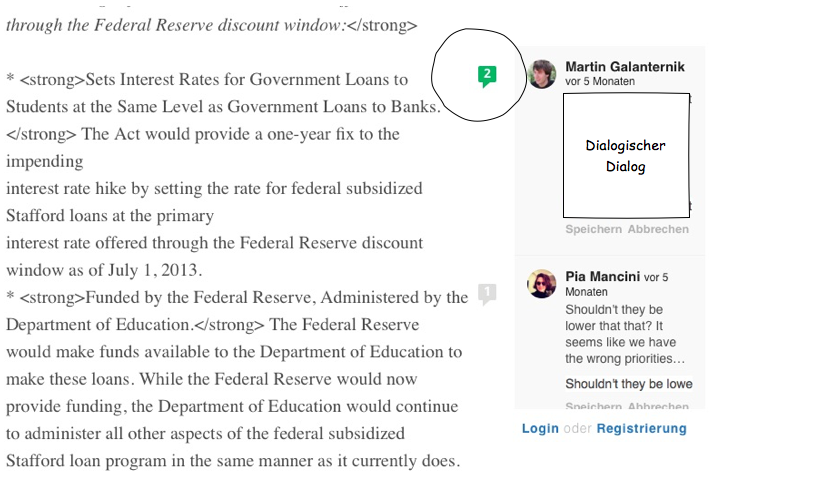
\includegraphics[width=1\textwidth]{img/democracyos.png}
\caption{Mögliche Anbindung der DSL an DemocracyOS}
\label{democracyos}
\end{figure}

Gezielte Angriffe

AllQuantor
EinsQuantor

\subsection{Faktencheck} % Simon

Einfachere Interpretation durch KI der Elementaraussagen ggü. komplexen Aussagen.  => Intelligenzverstärker durch einfachen Faktencheck

Zu Elementaraussae Tag-Cloud anzeigen mit Fakten (Open Data)

\begin{figure}[htbp]
\centering
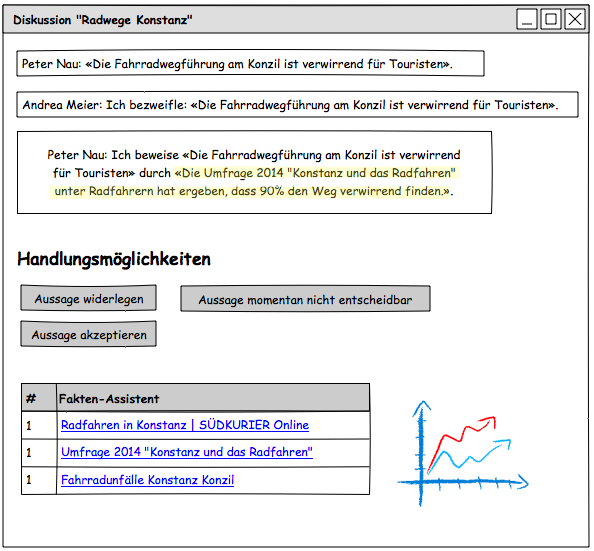
\includegraphics[width=1\textwidth]{img/faktencheck.png}
\caption{Faktencheck mit der DSL}
\label{faktencheck}
\end{figure}

Whatson versteht Elementaraussagen

\section{Politischer Unterrichtsdiskurs} % Tobi



% ============================ CHAPTER
\chapter{Fazit und Ausblick} % Tobi


Zusammenfassung

Selbstkritik

Ausblick

 
% ============================ ENDE HAUPTTEIL







% ============================ LITERATURVERZEICHNIS
\begin{singlespace}
\begin{thebibliography}{9}

\bibitem[Ort15]{OrtnerDL}
  Prof. Dr. Erich Ortner,
  \emph{Einf{\"u}hrung in die Dialogische Informatik},
  HTWG Präsentation,
  2015.
  
\bibitem[Dem15]{DemocracyOS}
  The DemocracyOS Foundation,
  \emph{DemocracyOS - Power in your hands},
  \url{http://democracyos.org},
  besucht am 25.06.2015.

\bibitem[Ecl15]{Xtext}
  The Eclipse Foundation,
  \emph{Xtext - Language Development Made Easy!},
  \url{https://eclipse.org/Xtext/},
  besucht am 25.06.2015.

\end{thebibliography}
\end{singlespace}
% ============================ ENDE LITERATURVERZEICHNIS



\end{document}

